\chapter{Unclear age pattern, requiring expert priors: premenstrual syndrome}
\label{applications-priors_knots_select}

Epidemiological data without clear age patterns are a reoccurring
theme in the GBD 2010 Study.  Unclear age patterns make expert priors
essential in the modeling process.  However, such cases are very
sensitive to the choice of prior assumptions, as shown in the
following example of premenstrual syndrome (PMS) in Western Europe.

PMS is a common cyclic disorder that affects women of reproductive
years during the period between ovulation and the onset of menses.
More than $200$ behavioral, psychological, and physical symptoms have been
associated with PMS, the most common being irritability, tension,
depression, bloating, weight gain, and food cravings.  The exact causes
of PMS are unknown, with no consistent
treatment option available. \cite{dickerson_premenstrual_2003, singh_incidence_1998,
  goodale_alleviation_1990}

A meta-analysis of data from a systematic review of the descriptive
epidemiology of PMS yielded $74$ prevalence
data points, of which $18$ were from Western Europe.  As seen from
figure~\ref{fig:app-pms_data}, the data are noisy, with overlapping and
heterogeneous age-groups that show no clear age pattern.

    \begin{figure}[h]
        \begin{center}
            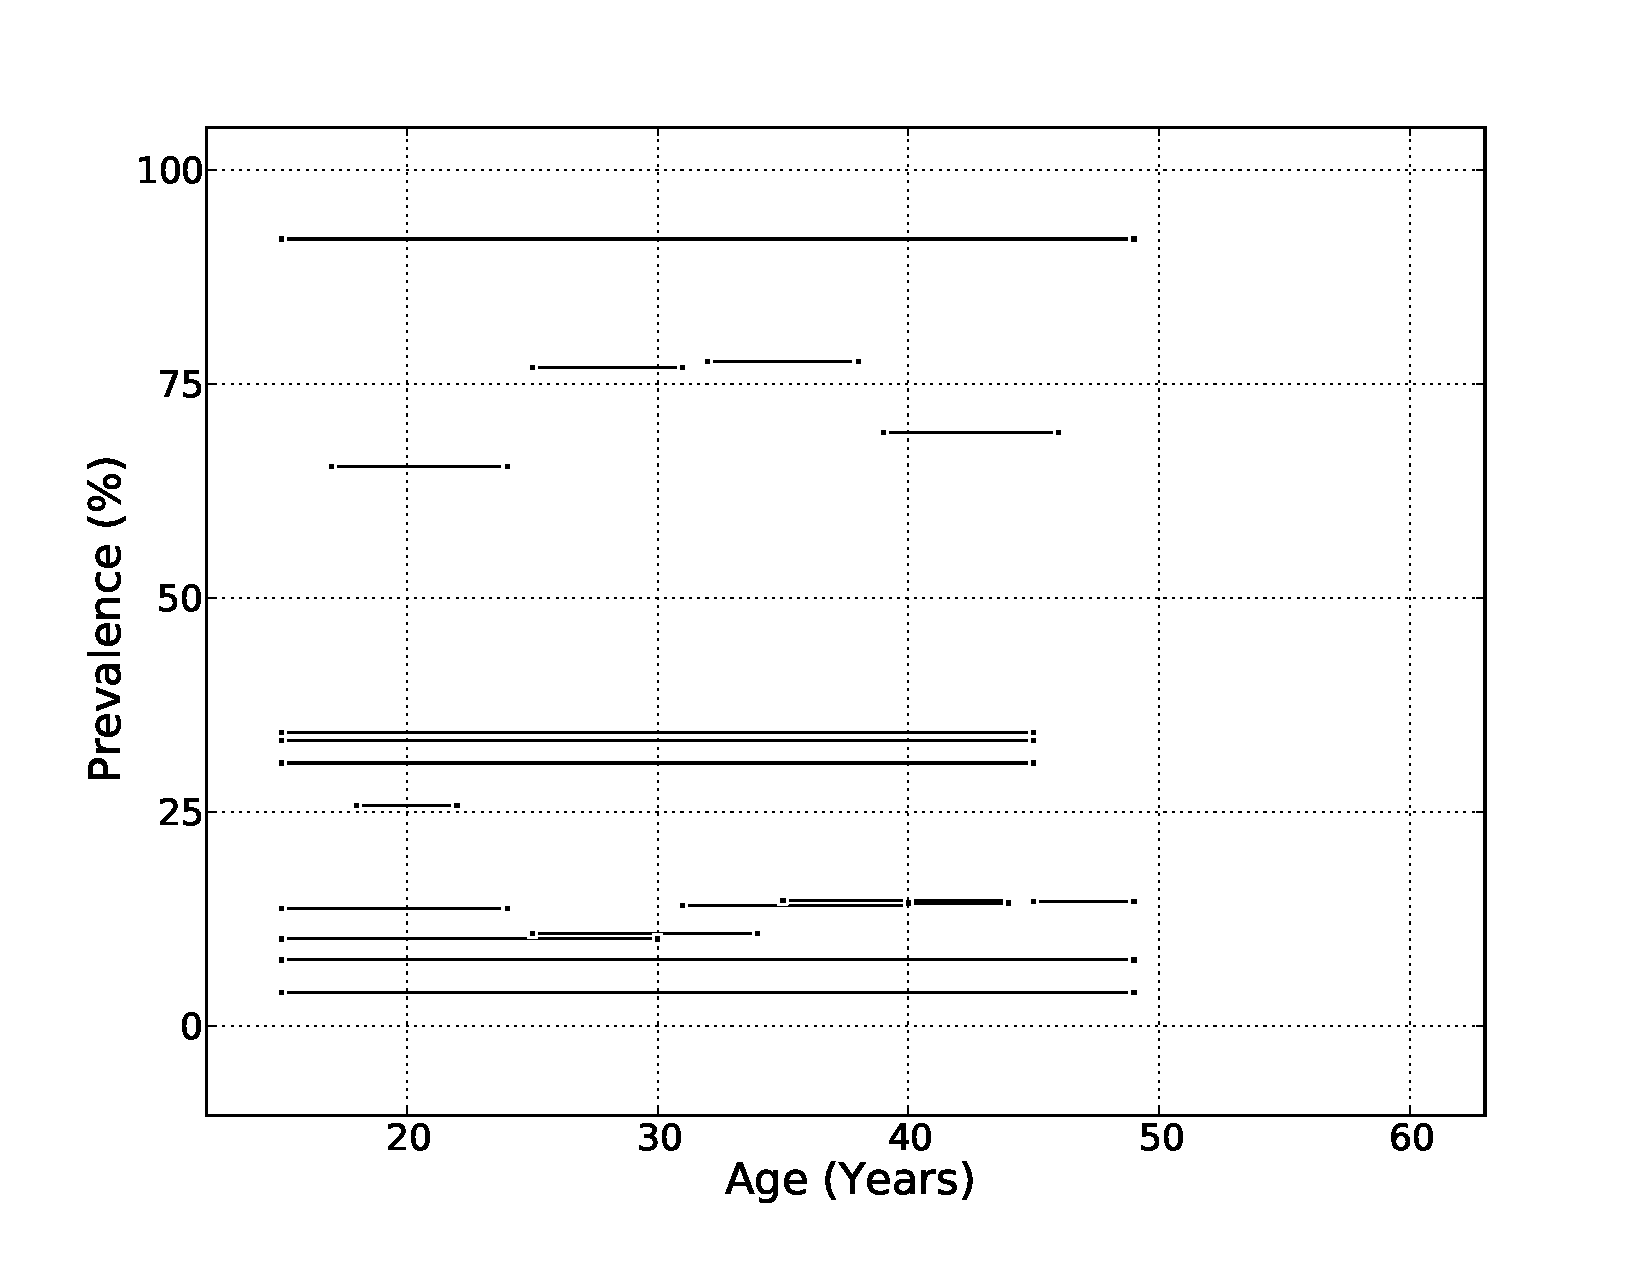
\includegraphics[width=\textwidth]{pms-data.pdf}
            \caption{Prevalence data for women with PMS
              in Western Europe.}
        \end{center}
        \label{fig:app-pms_data}
    \end{figure}

%% \section{Priors on level} \label{sec:app-priors on level}

In the absence of clear age patterns in the systematic review data
points, modeling decisions about knot location, age pattern levels, and
direction of age pattern trends have substantial influence on the estimates of
disease prevalence.  These decisions can also have unintended
consequences, as discussed in chapter~\ref{theory-age_pattern_model}.
To illustrate the effects, we fitted models with a variety of choices
about knot location, level values outside the measured age
intervals, and direction of age pattern trends.  Conducting a sensitivity analysis
like this is important when modeling sparse and noisy data.

As the prevalence data plotted in figure~\ref{fig:app-pms_data} show,
systematic review collected no data on population prevalence for women
younger than age $15$ or older than age $50$.  Since PMS is a disorder
related to the female reproductive cycle, it follows that data outside
this age range are not present for biological reasons.  However, this
information is not part of the spline model unless the modeler
explicitly includes it.  If no priors are included to inform estimates
in the young and old, then they are extrapolated from the levels where
there are data, as seen in figure~\ref{fig:app-pms prios_on_level}.
Here expert knowledge is needed to inform the model that cases are not
expected outside the age range where they have been measured.

    \begin{figure}
        \begin{center}
            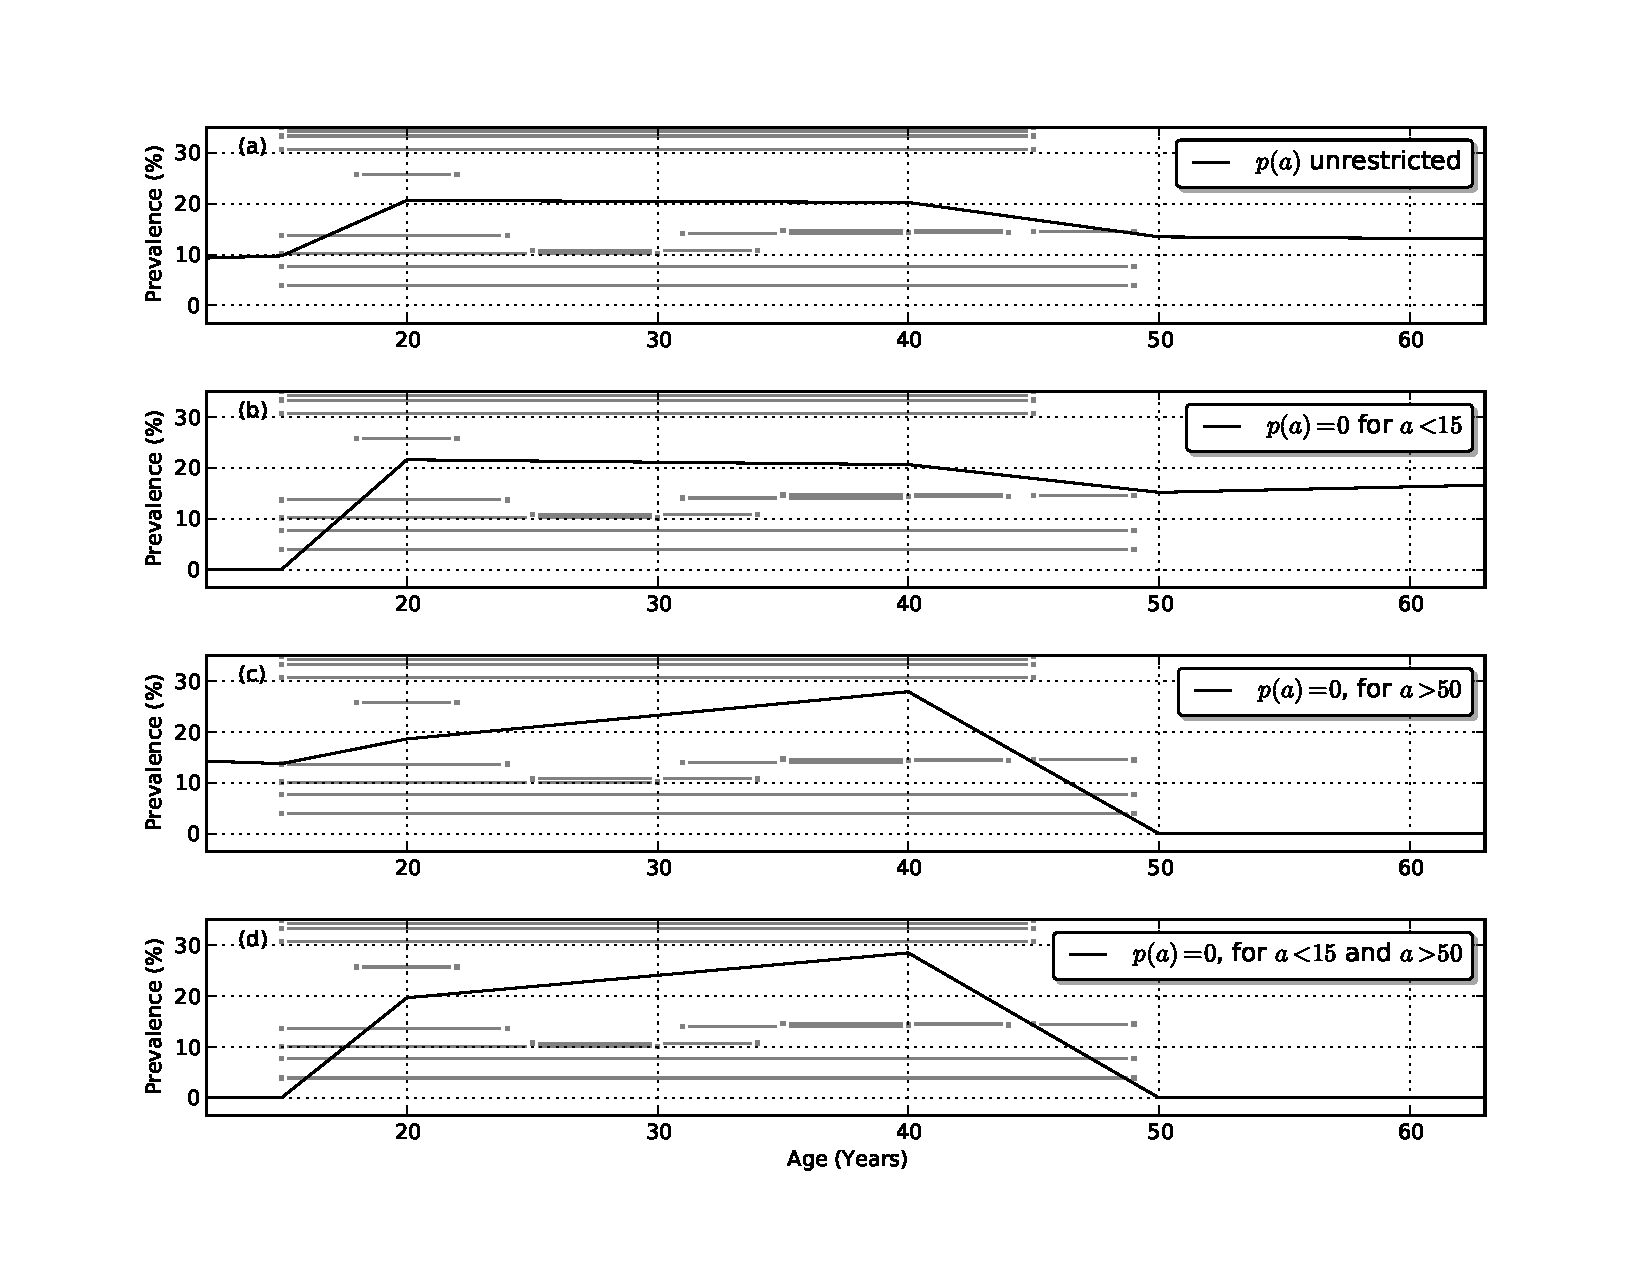
\includegraphics[width=\textwidth]{pms-priors.pdf}
        \end{center}
        \caption[Four estimates of age-specific PMS prevalence with
          different priors on prevalence in young and old ages]{Four
          estimates of age-specific PMS prevalence with different
          priors on prevalence in young and old ages.  Systematic
          review produced sparse and noisy data, shown here for
          Western Europe.  (a) Without a level prior to inform the
          model that prevalence data are not present outside 
          ages $15$--$50$ for biological reasons, estimates outside the
          ages measured are extrapolated from inside.  Restricting
          prevalence to $0$ changes the prevalence estimates
          substantially. (b) The effect of assuming $p(a) = 0$ for
          $a<15$, (c) the effect of assuming $p(a) = 0$ for $a>50$,
          and (d) the effect of assuming $p(a) = 0$ for $a<15$ and
          $a>50$ all change the estimates inside and outside the
          observed data ages.}
        \label{fig:app-pms prios_on_level}
    \end{figure}

%% \section{Knot location}

As described in
section~\ref{theory-age_group_model-overlapping_data}, we model
age-specific hazards with splines, using knots to partition the age
range into intervals.  Models with ample data and clear age patterns
are not very sensitive to knot choice.  However, with sparse and
noisy data without a clear age pattern, the number and location of
knots can influence the model results substantially.  We explored this
by fitting models with a variety of knots to the PMS data set, as seen
in figure~\ref{fig:app-pms knot_loc}.  Choosing the number and
location of knots a priori using expert knowledge allows the user to
determine critical features of the model in a principled way.

    \begin{figure}
        \begin{center}
            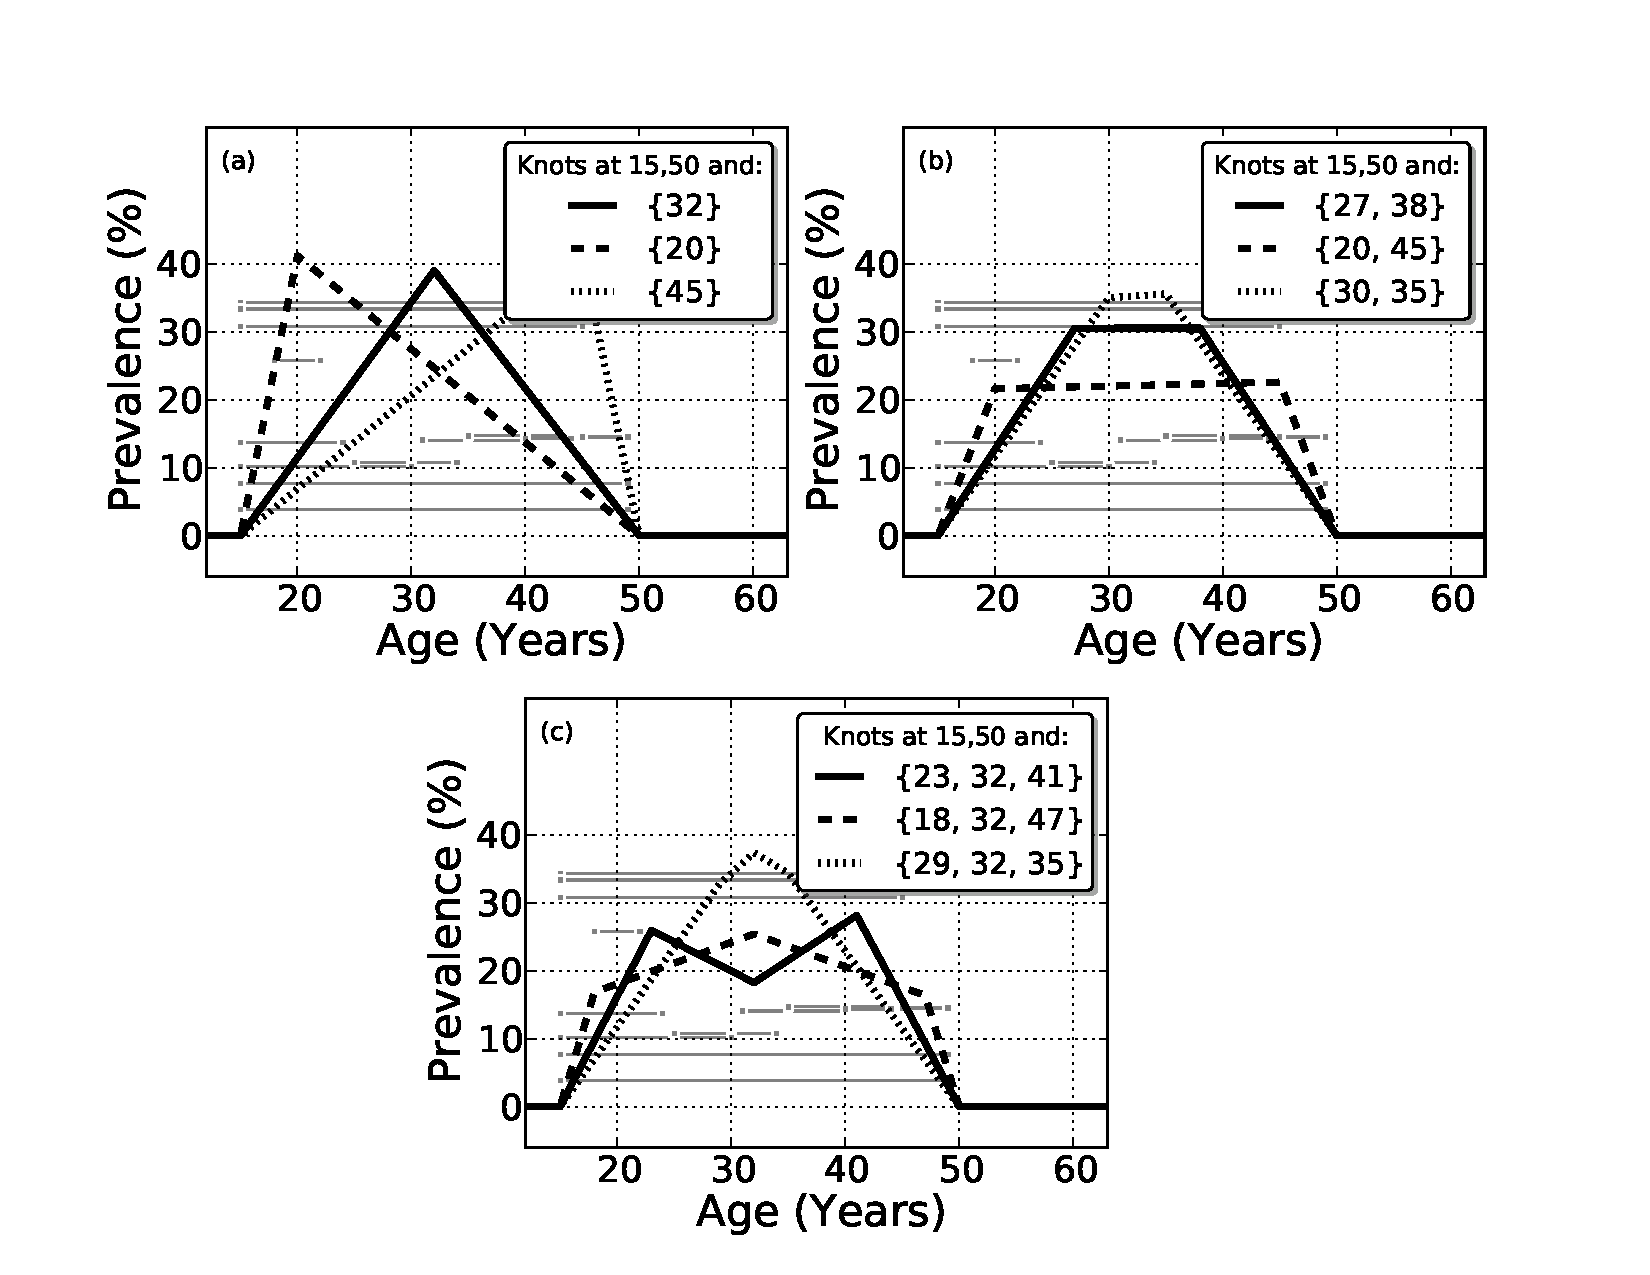
\includegraphics[width=\textwidth]{pms-knot_location.pdf}
        \end{center}
        \caption[Estimate of age-specific PMS prevalence for spline
          models with a variety of knots]{Estimate of age-specific PMS
          prevalence for spline models with a variety of knots.  All
          panels have knots at $\{0, 15, 50, 100\}$ and vary the number
          and location of knots between the ages of $15$ and $50$ to show
          the sensitivity of knot selection in sparse and noisy data
          without a clear age pattern. (a) With $1$ additional knot, the
          placement at age $20$, $32$, or $45$ gives markedly different
          estimates of PMS prevalence in Western Europe.  (b) With $2$
          knots at $\{27, 38\}$, $\{20, 45\}$, or $\{30, 35\}$, the
          differences are also clear and predictable. (c) With $3$ knots
          at locations $\{23, 32, 41\}$, $\{18, 32, 47\}$, or $\{29, 32,
          35\}$, it appears that the data are too sparse and noisy to
          support a consistent age pattern.}
        \label{fig:app-pms knot_loc}
    \end{figure}

%% \section{Priors on monotonicity}
Another common prior for age patterns is the belief that the
epidemiological parameter increases or decreases over a certain age
range.  As seen in figure~\ref{fig:app-pms dir}, priors on
monotonicity between the critical ages of $25$ and $40$ have a large
effect on the prevalence estimate for Western Europe.

    \begin{figure}
        \begin{center}
            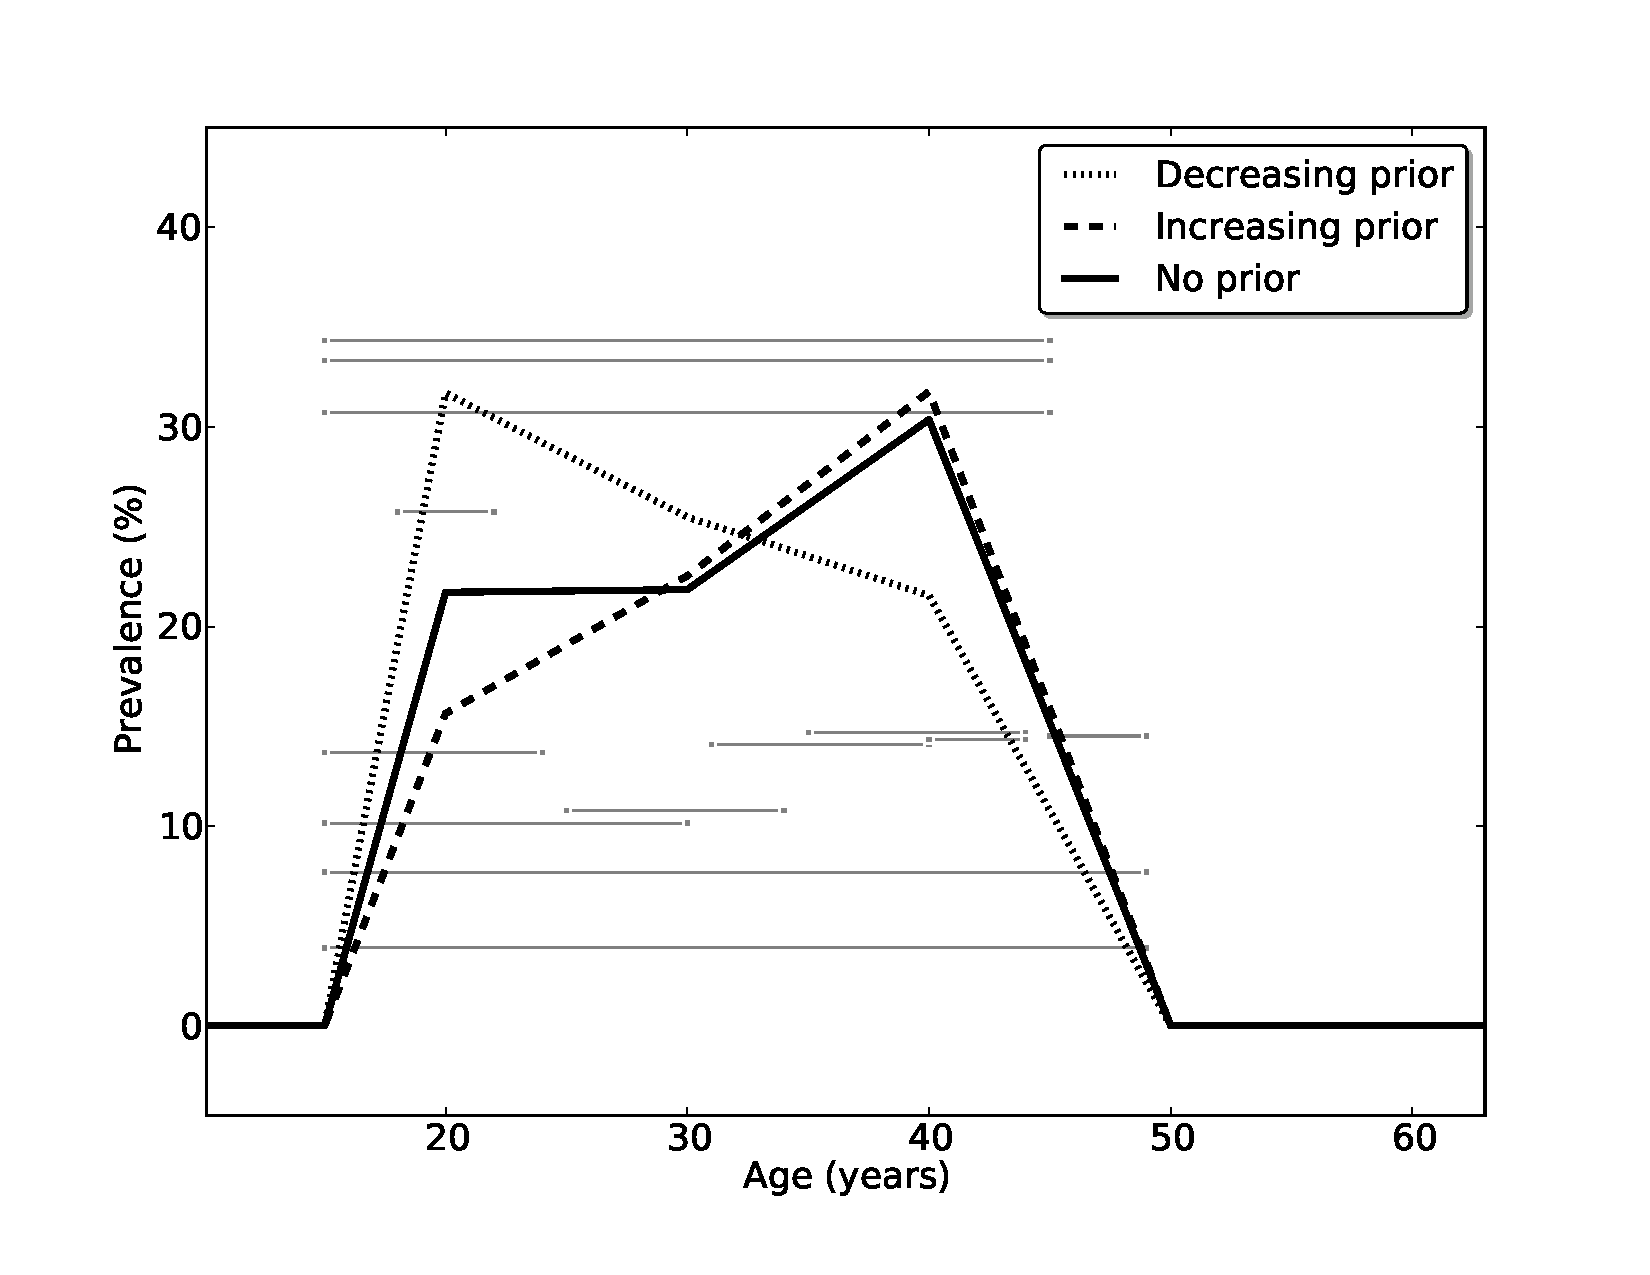
\includegraphics[width=\textwidth]{pms-direction.pdf}
        \end{center}
        \caption[Estimates of age-specific PMS prevalence for spline
          models with a variety of monotonicity priors]{Estimates of
          age-specific PMS prevalence for spline models with a variety
          of monotonicity priors. Between the ages of $25$ and $40$, the prior
          on monotonicity makes a large impact on the prevalence
          estimates for women in Western Europe with PMS.}
        \label{fig:app-pms dir}
    \end{figure}

Knot selection and priors on level and monotonicity play an important
role in the modeling process and in the sensitivity analysis.
However, when the data are not sufficient to understand the age
pattern, the model compensates by producing estimates with large
uncertainty, as seen in figure~\ref{fig:app-pms best}.  This estimate
comes from a model with knots at $\{0, 15, 20, 30, 40, 50, 100\}$, no
prior on monotonicity, and a prior on level to restrict prevalence to
be $0$ outside the age range $15$--$50$.

This example has identified an area of future research.  The model does
not have enough data to inform an age pattern because the descriptive
epidemiology of PMS is quite uncertain: some studies say almost all women
experience it and some studies say none do.  In such cases, making the
most informed decisions possible (such as restricting the model to
ages $15$--$50$ for biological reasons) and accepting a large uncertainty
interval reveal the truth: we just don't know.

    \begin{figure}
        \begin{center}
            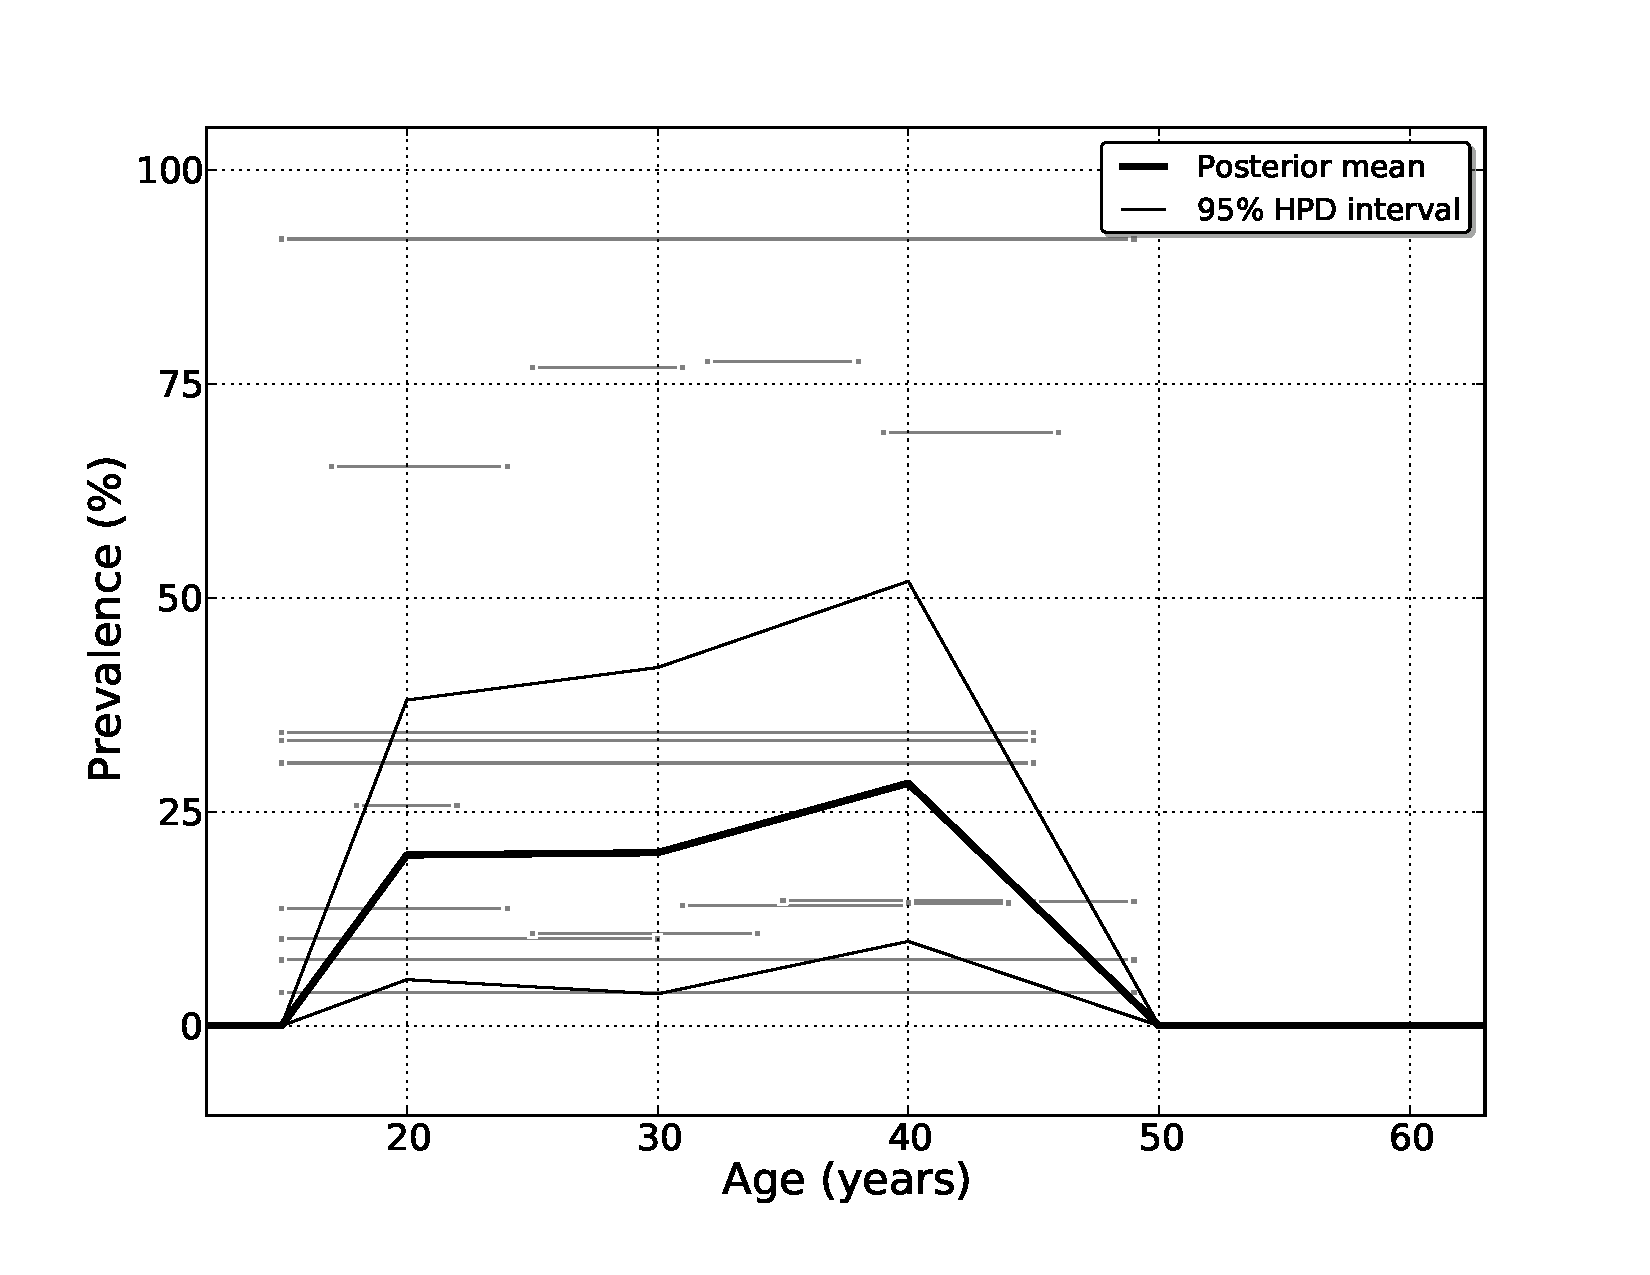
\includegraphics[width=\textwidth]{pms-best_model.pdf}
        \end{center}
        \caption{Prevalence estimates for women
          in Western Europe with PMS.}
        \label{fig:app-pms best}
    \end{figure}









